\documentclass{beamer}
\usepackage[utf8]{inputenc}

\usetheme{Madrid}
\usecolortheme{default}
\usepackage{amsmath,amssymb,amsfonts,amsthm}
\usepackage{mathtools}
\usepackage{txfonts}
\usepackage{tkz-euclide}
\usepackage{listings}
\usepackage{adjustbox}
\usepackage{array}
\usepackage{gensymb}
\usepackage{tabularx}
\usepackage{gvv}
\usepackage{lmodern}
\usepackage{circuitikz}
\usepackage{tikz}
\usepackage{graphicx}

\setbeamertemplate{page number in head/foot}[totalframenumber]

\usepackage{tcolorbox}
\tcbuselibrary{minted,breakable,xparse,skins}



\definecolor{bg}{gray}{0.95}
\DeclareTCBListing{mintedbox}{O{}m!O{}}{%
  breakable=true,
  listing engine=minted,
  listing only,
  minted language=#2,
  minted style=default,
  minted options={%
    linenos,
    gobble=0,
    breaklines=true,
    breakafter=,,
    fontsize=\small,
    numbersep=8pt,
    #1},
  boxsep=0pt,
  left skip=0pt,
  right skip=0pt,
  left=25pt,
  right=0pt,
  top=3pt,
  bottom=3pt,
  arc=5pt,
  leftrule=0pt,
  rightrule=0pt,
  bottomrule=2pt,
  toprule=2pt,
  colback=bg,
  colframe=orange!70,
  enhanced,
  overlay={%
    \begin{tcbclipinterior}
    \fill[orange!20!white] (frame.south west) rectangle ([xshift=20pt]frame.north west);
    \end{tcbclipinterior}},
  #3,
}
\lstset{
    language=C,
    basicstyle=\ttfamily\small,
    keywordstyle=\color{blue},
    stringstyle=\color{orange},
    commentstyle=\color{green!60!black},
    numbers=left,
    numberstyle=\tiny\color{gray},
    breaklines=true,
    showstringspaces=false,
}
%------------------------------------------------------------
%This block of code defines the information to appear in the
%Title page
\title %optional
{4.2.9}
\date{september 12,2025}
%\subtitle{A short story}

\author % (optional)
{EE25BTECH11006 - ADUDOTLA SRIVIDYA}

\begin{document}

\frame{\titlepage}

\begin{frame}{Question}
Find the direction and normal vector for the line 
\begin{align}
    x + y = 4
\end{align}
\end{frame}

\begin{frame}{Theoretical Solution}
The line can be written as
\begin{align}
    x + y = 4
\end{align}
Let
\begin{align}
    \vec{x} = \myvec{x \\ y}, \quad
    \vec{n^T} = \myvec{1 & 1}, \quad
    c = 4
\end{align}
Thus, the line equation is
\begin{align}
    \vec{n^T}\vec{x} = c
\end{align}
where $\vec{n}$ is the normal vector.
\end{frame}

\begin{frame}{Direction Vector}
The direction vector of the line can be found by observing the normal vector.
\begin{align}
\vec{m} = \myvec{-1 \\ 1}
\end{align}


This is true because if the director vector is represented as 
\begin{align}
\vec{m}  = \myvec{1 \\ m}    
\end{align}
then the normal vector can be represented as 
\begin{align}
\vec{n} = \myvec{-m \\ 1}
\end{align}
\end{frame}

\begin{frame}{Verification}
This can be verified by the following equation:
\begin{align}
\vec{n^T}\vec{m} = 0
\end{align}

\begin{align}
\myvec{1 & 1}\myvec{-1 \\ 1} = 0
\end{align}\\    
\end{frame}

\begin{frame}{Final Answer}
\begin{itemize}
    \item Normal vector: $\vec{n} = \myvec{1 \\ 1}$
    \item Direction vector: $\vec{m} = \myvec{-1 \\ 1}$
\end{itemize}
\end{frame}

\begin{frame}[fragile]{C code}
\begin{lstlisting}
#include <stdio.h>
int dot_product(int a[2], int b[2]) {
return a[0]*b[0] + a[1]*b[1];
}
int is_orthogonal(int a[2], int b[2]){
return dot_product(a,b) == 0;
}
double line_equation(double x) {
return (4.0 - 1.0*x)/1.0;
}
\end{lstlisting}
\end{frame}

\begin{frame}[fragile]{cpython code}
\begin{lstlisting}
import sys
import ctypes
import numpy as np
import matplotlib.pyplot as plt
# Load C library
c_lib = ctypes.CDLL('./formula.so')
c_lib.line_vectors.argtypes = [
    ctypes.POINTER(ctypes.c_float),  
    ctypes.POINTER(ctypes.c_float),  
    ctypes.c_float, ctypes.c_float
]
c_lib.line_vectors.restype = None  
\end{lstlisting}
\end{frame}

\begin{frame}[fragile]{cpython code}
\begin{lstlisting} 
# For line: x + y = 4
a, b, c = 1.0, 1.0, 4.0
normal = np.zeros(2, dtype=np.float32)
direction = np.zeros(2, dtype=np.float32)

c_lib.line_vectors(
    normal.ctypes.data_as(ctypes.POINTER(ctypes.c_float)),
    direction.ctypes.data_as(ctypes.POINTER(ctypes.c_float)),
    ctypes.c_float(a), ctypes.c_float(b)
)

print("Normal Vector:", normal)
print("Direction Vector:", direction)

\end{lstlisting}
\end{frame}

\begin{frame}[fragile]{cpython code}
\begin{lstlisting}
# Plot line
x = np.linspace(-1, 6, 100)
y = (c - a*x)/b
plt.plot(x, y, label="x+y=4")
# Plot normal at (2,2)
P = np.array([2, 2])
plt.quiver(P[0], P[1], normal[0], normal[1], angles='xy', scale_units='xy', scale=1, color='r', label='Normal')
plt.quiver(P[0], P[1], direction[0], direction[1], angles='xy', scale_units='xy', scale=1, color='g', label='Direction')
plt.xlabel('$x$')
plt.ylabel('$y$')
plt.legend()
plt.grid(True)
plt.axis('equal')
plt.savefig("figs/Plot_P.png")
plt.show()
\end{lstlisting}
\end{frame}

\begin{frame}[fragile]{pure python code}
\begin{lstlisting}
import numpy as np
import matplotlib.pyplot as plt

# Define the line equation x + y = 4
x_vals = np.linspace(-2, 6, 400)
y_vals = 4 - x_vals

# Normal and direction vectors
n = np.array([1, 1])
d = np.array([1, -1])
\end{lstlisting}
\end{frame}

\begin{frame}[fragile]{pure python code}
\begin{lstlisting}
# Point on the line
point_on_line = np.array([2, 2])

# Plot the line
plt.plot(x_vals, y_vals, label='Line: $x + y = 4$', color='blue')

# Normal vector
plt.quiver(point_on_line[0], point_on_line[1], n[0], n[1],
           angles='xy', scale_units='xy', scale=1, color='red', label='Normal Vector')

# Direction vector
plt.quiver(point_on_line[0], point_on_line[1], d[0], d[1],
           angles='xy', scale_units='xy', scale=1, color='orange', label='Direction Vector')
\end{lstlisting}
\end{frame}

\begin{frame}[fragile]{pure python code}
\begin{lstlisting}
# Annotate
plt.scatter(point_on_line[0], point_on_line[1], color='black')
plt.annotate('Point on line (2, 2)', (2, 2), textcoords="offset points",
             xytext=(10,-10), ha='center')
plt.annotate('Normal [1, 1]', (3, 3), textcoords="offset points",
             xytext=(10,10), color='red')
plt.annotate('Direction [1, -1]', (3, 1), textcoords="offset points",
             xytext=(10,-20), color='orange')
\end{lstlisting}
\end{frame}


\begin{frame}[fragile]{pure python code}
\begin{lstlisting}
# Axes
ax = plt.gca()
ax.spines['left'].set_position('zero')
ax.spines['bottom'].set_position('zero')
ax.spines['right'].set_color('none')
ax.spines['top'].set_color('none')

plt.xlabel('$x$')
plt.ylabel('$y$')
plt.legend(loc='best')
plt.grid(True)
plt.axis('equal')

plt.savefig('fig6.png')
plt.show()
\end{lstlisting}
\end{frame}

\begin{frame}{Plot}
\begin{figure}[H]
\centering
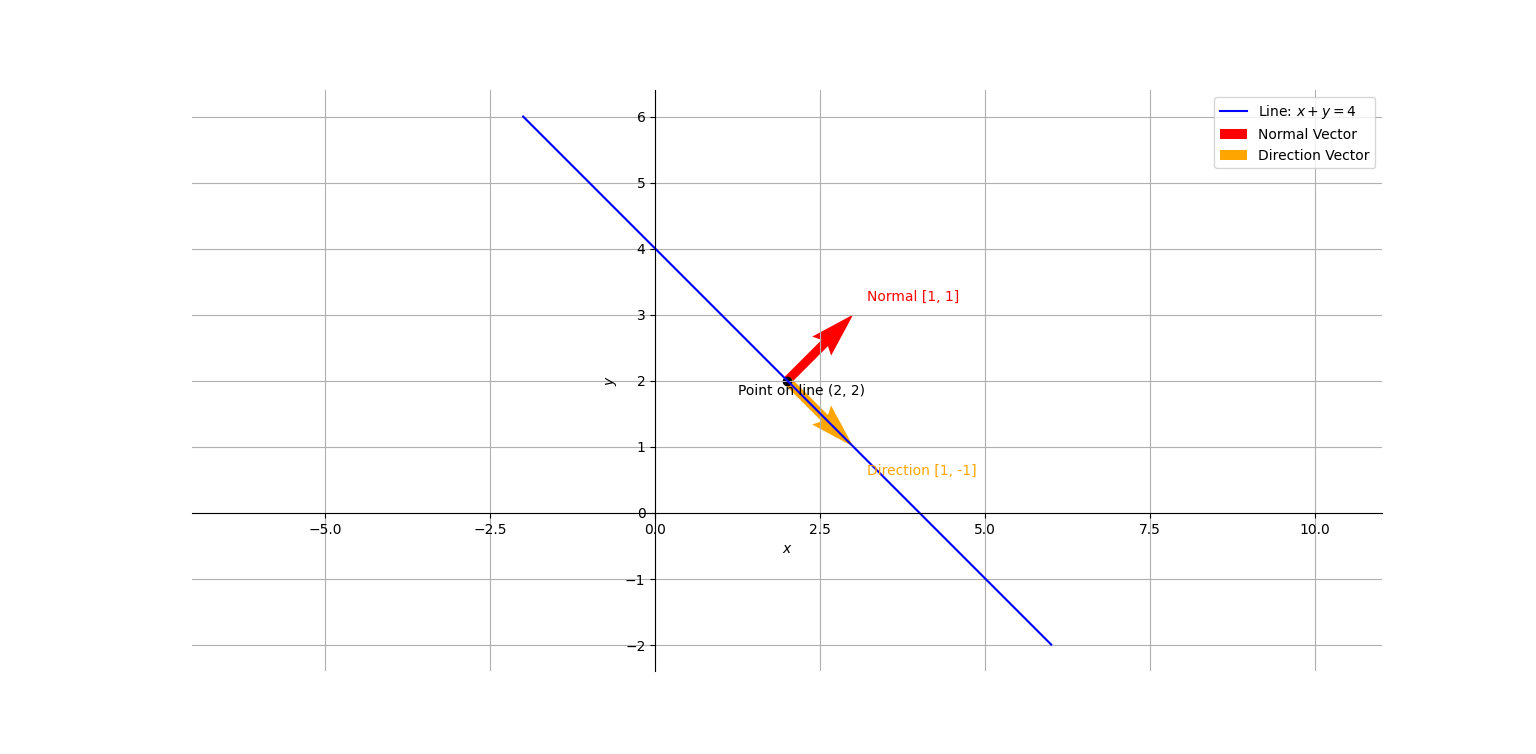
\includegraphics[width=0.65\linewidth]{figs/fig6.png}
\caption{Line $x+y=4$ with normal and direction vectors}
\end{figure}
\end{frame}

\end{document}